% ==============================================================================
% Relatorio Final - Projeto de Aprendizado de Maquina (UFSCar / DComp, 2026)
% Compilar com pdfLaTeX + BibTeX (ex.: Overleaf usando relatorio_overleaf.zip).
% Limite: maximo 4 paginas em coluna dupla, excluindo Referencias.
% ==============================================================================
\documentclass[10pt, conference, compsocconf]{IEEEtran}

\usepackage[utf8]{inputenc}
\usepackage[T1]{fontenc}
\usepackage[brazil]{babel}
\usepackage{amsmath}
\usepackage{amssymb}
\usepackage{graphicx}
\usepackage{booktabs}
\usepackage{array}
\usepackage{multirow}
\usepackage{cite}
\usepackage{url}
\usepackage{microtype}
\usepackage{placeins}

\renewcommand{\topfraction}{0.90}
\renewcommand{\bottomfraction}{0.65}
\renewcommand{\textfraction}{0.08}
\renewcommand{\floatpagefraction}{0.75}
\setcounter{topnumber}{3}
\setcounter{bottomnumber}{2}
\setcounter{totalnumber}{4}
\setlength{\textfloatsep}{7pt plus 2pt minus 2pt}
\setlength{\floatsep}{6pt plus 2pt minus 2pt}
\setlength{\intextsep}{7pt plus 2pt minus 2pt}

\renewcommand{\abstractname}{Resumo}
\renewcommand{\IEEEkeywordsname}{Palavras-chave}
\addto\captionsbrazil{%
  \renewcommand{\abstractname}{Resumo}%
  \renewcommand{\IEEEkeywordsname}{Palavras-chave}%
  \renewcommand{\figurename}{Figura}%
  \renewcommand{\tablename}{Tabela}%
  \renewcommand{\refname}{Refer\^{e}ncias}%
}
\AtBeginDocument{%
  \renewcommand{\abstractname}{Resumo}%
  \renewcommand{\IEEEkeywordsname}{Palavras-chave}%
  \renewcommand{\figurename}{Figura}%
  \renewcommand{\tablename}{Tabela}%
  \renewcommand{\refname}{Refer\^{e}ncias}%
}

\hyphenation{des-ba-lan-ce-a-men-to re-com-pra hi-e-rar-qui-co}

\begin{document}

\title{Previsão de Engajamento e Churn de Clientes no Varejo com Aprendizado de Máquina}

\author{%
\IEEEauthorblockN{Felipe Rodrigues Bastos}
\IEEEauthorblockA{Departamento de Computação (DComp)\\
Universidade Federal de São Carlos (UFSCar)\\
Sorocaba, São Paulo, Brasil -- RA: 815406\\
E-mail: felipe.bastos@estudante.ufscar.br}
\and
\IEEEauthorblockN{João Henrique de Camargo Brants}
\IEEEauthorblockA{Departamento de Computação (DComp)\\
Universidade Federal de São Carlos (UFSCar)\\
Sorocaba, São Paulo, Brasil -- RA: 802553\\
E-mail: joaobrants@estudante.ufscar.br}
}

\maketitle

\begin{abstract}
No varejo físico, não há cancelamento formal de conta: o cliente simplesmente reduz visitas até parar de comprar. Este artigo investiga a classificação multiclasse do engajamento futuro de clientes da rede VAI Store nos 90 dias após 30/09/2024, com 59.945 consumidores no treino e 25.691 no teste, com forte desbalanceamento entre classes (25,88\% Ativo, 7,96\% Desacelerando, 2,35\% Dormente e 63,81\% Churn). A limpeza sem vazamento de 397.625 transações revelou dois regimes (dia único versus recorrente) e mostrou que filtros por intervalo interquartil (IQR) removem 55,9\% dos clientes Dormentes. Criamos 170 atributos temporais com o modelo probabilístico BG/NBD, comparamos 11 classificadores e propusemos uma arquitetura hierárquica em três etapas com CatBoost nativo, calibração, máscara estrutural e ajuste de decisão Plug-in para F1-macro. Em validação cruzada de 10 partições, o comitê atingiu F1-macro de 0,4398 (desvio-padrão de 0,0049), AUC-OvR de 0,7880, Log-Loss de 0,7424 e 0,44075 no Public Leaderboard.
\end{abstract}

\begin{IEEEkeywords}
Aprendizado de Máquina; Predição de Churn; Classificação Multiclasse; Desbalanceamento; F1-Macro; Comitês de Classificadores.
\end{IEEEkeywords}

\section{Introdução}
No varejo físico sem contrato ou assinatura, identificar quando um cliente deixará de comprar é desafiador porque não existe aviso prévio de saída~\cite{buckinx2005retail}. O consumidor apenas espaça mais as visitas até interromper as compras. Usando transações reais de 2024 da VAI Store, rede especializada com lojas de rua e em \textit{shoppings}, o objetivo deste trabalho é prever o nível de engajamento de cada cliente nos 90 dias seguintes à data de corte de 30/09/2024. As amostras dividem-se em quatro classes: \textbf{Classe~0 (Ativo)}, nova compra em até 1,2 vez o ciclo médio habitual; \textbf{Classe~1 (Desacelerando)}, atraso entre 1,2 e 2,0 vezes o ciclo; \textbf{Classe~2 (Dormente)}, atraso acima de 2,0 vezes o ciclo; e \textbf{Classe~3 (\textit{Churn} Efetivo)}, nenhuma compra no trimestre futuro.

Esse cenário traz desafios práticos: a Classe~2 soma apenas 2,35\% dos casos, 53,10\% dos clientes compraram em um único dia sem histórico de retorno, existem ruídos nas vendas brutas e a regra padrão \textit{argmax} ignora classes menores. Assim, adotamos limpeza pré-corte sem vazamento, preservação dos clientes diante de filtros de \textit{outliers}, engenharia de 170 atributos com BG/NBD, modelo hierárquico com CatBoost e ajuste de limiares para F1-macro. A Seção~II revisa trabalhos relacionados; a Seção~III detalha dados e atributos; as Seções~IV e~V apresentam métodos e protocolo; a Seção~VI analisa os resultados; a Seção~VII descreve as submissões; e a Seção~VIII conclui.

\section{Trabalhos Relacionados}
Em bases sem contrato formal, Fader, Hardie e Lee~\cite{fader2005bgnbd} formularam o modelo BG/NBD para estimar a taxa esperada de compras e a probabilidade de atividade usando apenas recência, frequência e histórico do cliente. No varejo físico, Buckinx e Van den Poel~\cite{buckinx2005retail} ligam a redução de frequência a quedas recentes de gasto e maior variação entre visitas, enquanto Neslin et al.~\cite{neslin2006churn} mostram o impacto da janela de observação e da seleção de atributos nos modelos de \textit{churn}.

Em dados tabulares, Florestas Aleatórias~\cite{breiman2001rf} e métodos de \textit{Gradient Boosting}, como XGBoost~\cite{chen2016xgboost}, LightGBM~\cite{ke2017lightgbm} e CatBoost~\cite{prokhorenkova2018catboost} (com codificação ordenada de categóricas), lideram em desempenho e ganham estabilidade em comitês diversos~\cite{caruana2004ensemble,hastie2009esl}. Sob forte desbalanceamento, técnicas como SMOTE~\cite{chawla2002smote} e pesos na perda distorcem as probabilidades previstas~\cite{guo2017calibration}. Por isso, Lipton et al.~\cite{lipton2014f1} mostram que maximizar o F1 funciona melhor ajustando limiares sobre probabilidades calibradas, e Silla e Freitas~\cite{silla2011hierarchical} formalizam a divisão hierárquica de classes adotada neste trabalho.

\section{Dados e Pré-processamento}

\subsection{Limpeza Transacional e Análise Exploratória}
As bases somam 59.945 clientes no treino (\texttt{train.csv}), 25.691 no teste (\texttt{test.csv}), 557.294 registros de venda (\texttt{vendas\_dirty.csv}) e 6.499 produtos (\texttt{produto\_dirty.csv}). Os 14 atributos pré-computados resumem número de compras, itens, faturamento, tíquete médio, recência, antiguidade, ciclo médio e desvio, variedade de SKUs e categorias, proporção a granel, filial e tendência de gasto. Para evitar vazamento após 30/09/2024, recuperamos 1.113 datas corrompidas via \texttt{COD\_ATEND} e filtramos compras entre 01/01/2024 e 30/09/2024 (402.420 linhas). Removemos 3.985 registros sem CPF, 367 duplicatas exatas e 443 por \texttt{COD\_VENDA}; corrigimos 812 filiais via \texttt{COD\_FILIAL}; e tratamos 8.875 quantidades, 8.695 faturamentos inválidos e 5 SKUs sem categoria, chegando a \textbf{397.625 vendas limpas}. Na Figura~\ref{fig:eda}b, o volume sobe de 37.214 transações em janeiro até o pico de 51.206 em agosto (+37,6\%), fechando setembro com 47.034.

No treino há 15.513 Ativos (25,88\%), 4.772 Desacelerando (7,96\%), 1.409 Dormentes (2,35\%) e 38.251 em Churn (63,81\%). Como ilustra a Figura~\ref{fig:eda}a, compradores de 1 único dia (53,10\% da base) apresentam 80,7\% de \textit{churn} e zero casos da Classe~2, pois não possuem ciclo de recompra. Entre clientes recorrentes (2+ dias, 46,90\%), o \textit{churn} cai para 44,7\% e todas as classes ocorrem. Como a janela futura é fixa em 90 dias, apenas quem tem ciclo curto consegue atrasar acima de 2,0 vezes o ciclo antes do fim da janela: no treino, a Classe~1 aparece até ciclos de 76,0 dias e a Classe~2 até 45,33 dias (média de 20,35 dias e 6,10 compras). Por filial (Figura~\ref{fig:eda}c), unidades de \texttt{RUA} (28.441 clientes) concentram mais recorrentes (50,8\% contra 43,4\%) e menor \textit{churn} (60,9\% contra 66,5\%), enquanto unidades em \texttt{SHOPPING} (31.504 clientes) têm tíquete médio 19\% maior (R\$ 14,49 contra R\$ 12,18).

\begin{figure}[!t]
\centering
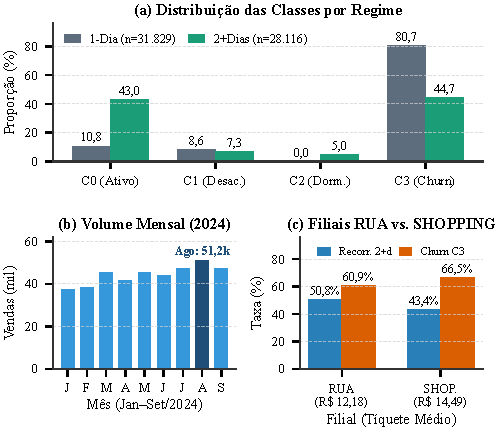
\includegraphics[width=0.92\columnwidth]{figs/fig1_eda.pdf}
\caption{Análise exploratória pré-corte: distribuição das classes por regime de frequência (a), volume mensal em 2024 (b) e comparação entre filiais (c).}
\label{fig:eda}
\end{figure}

\subsection{Outliers, Imputação e Engenharia de Atributos}
Na limpeza, verificamos que remover \textit{outliers} pelo critério clássico de 1,5 vez o intervalo interquartil (IQR) descartaria 32,7\% do treino e suprimiria \textbf{55,9\% da Classe~2}, confundindo clientes muito frequentes com ruído. Assim, mantivemos 100\% dos clientes. Nos algoritmos baseados em árvores, preservamos os ausentes de ciclo nativamente; para modelos lineares, SVM e MLP, aplicamos imputação pela mediana, indicadores de ausência, truncamento no quantil 0,995 e padronização robusta.

Construímos 170 atributos pré-corte em camadas. A \textbf{Camada~A} adiciona 32 razões sobre as tabelas principais, como atraso relativo, folgas frente a 1,2 e 2,0 vezes o ciclo e indicador de regime (46 variáveis ao todo). A \textbf{Camada~B} extrai 124 descritores do histórico limpo, cobrindo janelas de 30, 60 e 90 dias, variação entre últimos retornos (\texttt{gap\_delta\_ultimos}), razão entre penúltima visita e ciclo, preço/kg, SKU e categoria principais e sazonalidade semanal. Somamos ainda estimativas BG/NBD~\cite{fader2005bgnbd} (\texttt{nb\_p0} a \texttt{nb\_p3}) ajustadas por dobra (201 variáveis efetivas) e testamos um recorte com os 82 atributos de maior ganho.

\section{Materiais e Métodos}
Em Python 3.12 com Scikit-learn~\cite{pedregosa2011sklearn}, LightGBM, XGBoost, CatBoost, Imbalanced-learn e SciPy, testamos 11 algoritmos de diferentes famílias. Entre modelos lineares e de árvore, avaliamos Regressão Logística L2 ($C=0{,}5$), Regressão com \textit{Splines} ($C=0{,}3$, 5 nós), Linear SVM calibrado ($\alpha=10^{-3}$), Árvore de Decisão (profundidade 10, 50/folha), Florestas Aleatórias~\cite{breiman2001rf} e Extra Trees (160 árvores, 8/folha). Nos algoritmos neurais e de \textit{boosting}, incluímos MLP (camadas 64 e 32, $\alpha=0{,}01$), HistGradientBoosting (23 folhas, L2 $=5{,}0$), XGBoost~\cite{chen2016xgboost}, LightGBM~\cite{ke2017lightgbm} e CatBoost~\cite{prokhorenkova2018catboost}, usando \textit{Target Encoding} em 5 dobras nos modelos sem suporte categórico nativo.

Também testamos arquiteturas adaptadas ao problema. Primeiro, treinamos especialistas separados para clientes de 1 dia e de 2+ dias. Depois, adotamos uma decomposição hierárquica em três estágios~\cite{silla2011hierarchical}, prevendo em sequência se o cliente volta a comprar em 90 dias, se atrasa ao voltar e se esse atraso supera 2,0 vezes o ciclo, multiplicando essas probabilidades condicionais. No \textbf{CatBoost Hierárquico Nativo}, mantivemos essa divisão usando codificação ordenada em \texttt{sku\_principal\_1}, \texttt{cat\_principal\_1} e filial (profundidade 5 nos dois primeiros estágios e 4 no terceiro, taxa 0,045 e L2 de 10,0 e 12,0).

Como SMOTE~\cite{chawla2002smote} e pesos na perda descalibraram as probabilidades, mantivemos as proporções originais no treino e aplicamos três ajustes após a predição: calibração logística por temperatura~\cite{guo2017calibration}, máscara estrutural (zerando Classe~2 no regime de 1 dia e fora dos limites observáveis de ciclo) e a regra \textbf{Plug-in Expected Macro-F1}~\cite{lipton2014f1}. Em vez de escolher a classe mais provável via \textit{argmax}, que ignora as classes minoritárias, essa regra aplica multiplicadores e deslocamentos ajustados iterativamente sobre as probabilidades calibradas para maximizar o F1-macro esperado, sem consultar rótulos de teste. Por fim, combinamos os modelos via otimização SLSQP na Log-Loss~\cite{caruana2004ensemble}.

\section{Protocolo Experimental}
Os experimentos iniciais usaram validação cruzada estratificada em 5 partições; na etapa final, expandimos para \textbf{10 partições estratificadas} fixas e compartilhadas entre os modelos com 170 atributos e com o recorte Top~82. Essa mudança amplia o treino por dobra de 80\% para 90\% da base, o que ajuda especialmente nas classes raras, enquanto a predição final do conjunto de teste usa a média das probabilidades geradas pelas 10 dobras, reduzindo a variância. Todo ajuste dependente dos dados (imputadores, \textit{Target Encoding}, BG/NBD e parada antecipada interna com 10\% a 12\% do treino) ocorreu apenas dentro de cada dobra de treino. Para evitar sobreajuste no pós-processamento, validamos pesos do comitê (SLSQP), calibração e limiares \textit{Plug-in} em esquema aninhado (\textit{nested out-of-fold}): para cada dobra avaliada, esses parâmetros foram estimados nas outras 9 dobras e aplicados fora da amostra; somente na geração do arquivo de teste usamos a média dos pesos das 10 dobras e o pós-processamento ajustado sobre o conjunto OOF completo.

Na busca de hiperparâmetros com \texttt{RandomizedSearchCV} (3 dobras internas, métrica \texttt{neg\_log\_loss}), selecionamos para o LightGBM taxa de aprendizado 0,025, profundidade máxima 4, 15 folhas, mínimo de 180 amostras por folha, subamostragem de 85\% das linhas e 65\% das colunas e penalidades L1 $=5{,}0$ e L2 $=10{,}0$ (286 árvores médias); para o XGBoost, taxa 0,025, profundidade 4, peso mínimo 30, $\gamma=0{,}3$, subamostragem de 85\% das linhas e 80\% das colunas e L1 $=5{,}0$ / L2 $=10{,}0$ (341 árvores). Avaliamos F1-macro, AUC-OvR macro, PR-AUC, Log-Loss e Erro de Calibração Esperado (ECE), com testes de Friedman e Wilcoxon unilateral~\cite{demsar2006statistical}, validação adversarial treino-teste, simulação Monte Carlo (20 repetições) e \textit{bootstrap} ($n=7.707$ e $n=17.984$).

\section{Resultados}

\subsection{Estudos de Ablação}
\begin{table}[!t]
\centering
\caption{Ablações fora da amostra (5 partições, média $\pm$ desvio-padrão).}
\label{tab:ablacoes}
\scriptsize
\setlength{\tabcolsep}{1.7pt}
\begin{tabular}{@{}llccc@{}}
\toprule
\textbf{Exp.} & \textbf{Configuração} & \textbf{F1-Macro $\pm$ DP} & \textbf{AUC} & \textbf{Log-Loss} \\
\midrule
\multirow{3}{*}{Exp. 1}
 & IQR ($1{,}5\times$) + R. Forest & 0,4054 $\pm$ 0,0029 & 0,7527 & --$^\ast$ \\
 & Sem IQR + R. Forest & 0,4152 $\pm$ 0,0044 & 0,7578 & --$^\ast$ \\
 & Sem IQR + ausentes + Bayes & \textbf{0,4255 $\pm$ 0,0041} & \textbf{0,7806} & --$^\ast$ \\
\midrule
\multirow{4}{*}{Exp. 2}
 & Originais (14 atrib.) & 0,4331 $\pm$ 0,0042 & 0,7838 & 0,7469 \\
 & + Camada A (46 atrib.) & 0,4309 $\pm$ 0,0031 & 0,7842 & 0,7462 \\
 & + Camada B + BG/NBD & 0,4347 $\pm$ 0,0033 & \textbf{0,7864} & \textbf{0,7442} \\
 & Top 82 (LightGBM) & \textbf{0,4356 $\pm$ 0,0033} & 0,7861 & 0,7446 \\
\midrule
\multirow{5}{*}{Exp. 3}
 & Linha de base \textit{Argmax} & 0,3389 $\pm$ 0,0039 & \textbf{0,7859} & 0,7451 \\
 & SMOTE no treino & 0,3842 $\pm$ 0,0070 & 0,7818 & 0,7683 \\
 & Pesos \texttt{balanced} & 0,3983 $\pm$ 0,0046 & 0,7577 & 1,0354 \\
 & Pesos suav. ($\alpha=0{,}5$) & 0,4114 $\pm$ 0,0027 & 0,7778 & 0,8097 \\
 & Calib. + Másc. + \textbf{Plug-in} & \textbf{0,4361 $\pm$ 0,0052} & \textbf{0,7859} & \textbf{0,7447} \\
\bottomrule
\multicolumn{5}{l}{\scriptsize $^\ast$Log-Loss não mensurada na ablação inicial de pré-processamento.}
\end{tabular}
\end{table}

Na Tabela~\ref{tab:ablacoes}, remover o corte IQR aumentou o F1-macro em $+0{,}0098$ ao manter a Classe~2; somar tratamento nativo de ausentes e decisão Bayesiana chegou a 0,4255. No Experimento~2, expandir para 170 atributos baixou a Log-Loss de 0,7469 para 0,7442 (AUC 0,7864), e o recorte Top~82 alcançou 0,4356. Na Figura~\ref{fig:roc_imp}b, lideram por ganho no LightGBM \texttt{nb\_p0} (45,2 mil), \texttt{atraso\_zscore} (20,0 mil), \texttt{nb\_p3} (13,9 mil), \texttt{log\_nb\_p0} (12,4 mil), \texttt{ciclo\_medio\_dias} (9,2 mil), \texttt{janela\_frac\_c0} (9,1 mil) e \texttt{gap\_delta\_ultimos} (7,2 mil), porque medem a chance de retorno, o atraso atual frente ao histórico e o ritmo de recompra em 90 dias. No Experimento~3, \textit{argmax} caiu para 0,3389, enquanto SMOTE (0,3842) e pesos \texttt{balanced} (0,3983) degradaram a Log-Loss (1,0354); já o pós-processamento \textit{Plug-in} subiu para \textbf{0,4361 (+0,0972)} com Log-Loss de 0,7447.

\subsection{Comparação de Modelos, Testes Estatísticos e Public LB}
\begin{table}[!t]
\centering
\caption{Comparativo fora da amostra (ordenado por F1-macro com Plug-in F1).}
\label{tab:modelos}
\scriptsize
\setlength{\tabcolsep}{2.5pt}
\begin{tabular}{@{}lccc@{}}
\toprule
\textbf{Modelo / Arquitetura} & \textbf{F1-Macro $\pm$ DP} & \textbf{AUC} & \textbf{Log-Loss} \\
\midrule
\textbf{Comitê Linear (10 part.)$^\dagger$} & \textbf{0,4398 $\pm$ 0,0049} & \textbf{0,7880} & \textbf{0,7424} \\
Comitê Log-Odds (5 part.) & 0,4388 $\pm$ 0,0028 & 0,7875 & 0,7427 \\
XGBoost (parada antecipada) & 0,4372 $\pm$ 0,0027 & 0,7865 & 0,7440 \\
LightGBM (ajustado) & 0,4371 $\pm$ 0,0026 & 0,7865 & 0,7442 \\
CatBoost Hierárquico Nativo$^\dagger$ & 0,4370 $\pm$ 0,0042 & 0,7874 & 0,7432 \\
LightGBM (parada antecipada) & 0,4356 $\pm$ 0,0033 & 0,7861 & 0,7446 \\
Regressão Logística L2 & 0,4355 $\pm$ 0,0031 & 0,7857 & 0,7449 \\
Especialista LightGBM$^\dagger$ & 0,4353 $\pm$ 0,0050 & 0,7859 & 0,7440 \\
CatBoost (parada antecipada) & 0,4344 $\pm$ 0,0029 & 0,7870 & 0,7441 \\
Regressão com Splines (GAM) & 0,4333 $\pm$ 0,0047 & 0,7852 & 0,7456 \\
Rede Neural MLP & 0,4295 $\pm$ 0,0060 & 0,7823 & 0,7493 \\
Extra Trees & 0,4293 $\pm$ 0,0046 & 0,7822 & 0,7477 \\
HistGradientBoosting & 0,4283 $\pm$ 0,0061 & 0,7838 & 0,7468 \\
Florestas Aleatórias & 0,4258 $\pm$ 0,0056 & 0,7823 & 0,7486 \\
SVM Linear (SGD calibrado) & 0,4157 $\pm$ 0,0058 & 0,7528 & 0,7721 \\
Árvore de Decisão & 0,4072 $\pm$ 0,0071 & 0,7644 & 0,7939 \\
\bottomrule
\multicolumn{4}{l}{\scriptsize $^\dagger$Protocolo final em 10 partições estratificadas; demais em 5 partições.}
\end{tabular}
\end{table}

Na Tabela~\ref{tab:modelos}, \textit{Gradient Boosting} e Regressão Logística L2 superaram árvores isoladas, SVM, florestas paralelas e MLP. Friedman em 19 arquiteturas rejeitou igualdade (estatística $= 65{,}14$, $p = 2{,}95 \times 10^{-7}$), e Wilcoxon unilateral confirmou vantagem do comitê ($p = 0{,}0312$). Em 10 partições, o \textbf{CatBoost Hierárquico Nativo} liderou individualmente ($0{,}4370 \pm 0{,}0042$). Já o \textbf{Comitê Linear} alcançou F1-macro de \textbf{0,4398 $\pm$ 0,0049}, com AUC de 0,7880, Log-Loss de 0,7424 e ECE de 0,0025. Sua combinação reúne CatBoost Hierárquico Nativo (28,4\%), Regressão Logística (31,9\% entre os conjuntos de 82 e 170 atributos), Especialista LightGBM (13,3\%), LightGBM ajustado (11,4\%), XGBoost Hierárquico (8,2\%) e MLP (6,7\%). O escore ficou a 0,0009 do limite Bayesiano estimado ($0{,}4407 \pm 0{,}0026$), sem \textit{shift} treino-teste (AUC adversarial de 0,5007). No \textbf{\textit{Public Leaderboard}}, subimos de \textbf{0,43551} e \textbf{0,43294} (5 partições) para \textbf{0,44075} (Comitê Linear) e \textbf{0,43716} (CatBoost Hierárquico Nativo).

\subsection{Matrizes de Confusão, Classes e Subgrupos}
\begin{figure}[!t]
\centering
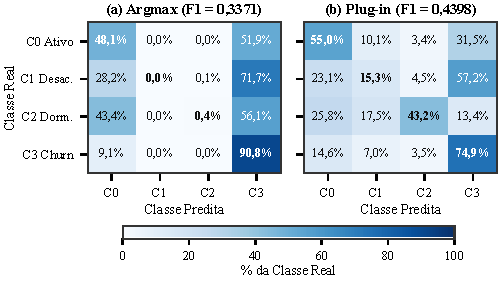
\includegraphics[width=0.98\columnwidth]{figs/fig2_matrizes_confusao.pdf}
\caption{Matrizes de confusão normalizadas fora da amostra do comitê final (10 partições): regra \textit{argmax} (a) versus pós-processamento Plug-in F1 (b).}
\label{fig:matrizes}
\end{figure}

Na Figura~\ref{fig:matrizes}, o \textit{argmax} zera a Classe~1 e acerta apenas 0,4\% da Classe~2; com o ajuste \textit{Plug-in}, a revocação da Classe~2 sobe para \textbf{43,2\%} e a da Classe~1 para 15,3\%, mantendo precisão de 78,6\% na Classe~3 (Tabela~\ref{tab:classes_subgrupos}). Nas curvas ROC-OvR (Figura~\ref{fig:roc_imp}a), a Classe~2 atinge AUC de 0,9445 por reunir clientes de ciclo curto e alta frequência, enquanto a Classe~1 (AUC 0,6659; F1 0,1462) sofre sobreposição entre Ativo e Churn. Nos subgrupos da Tabela~\ref{tab:classes_subgrupos}, clientes de 1 dia concentram 80,7\% de Churn e não possuem ciclo prévio, levando o modelo a concentrar previsões em Churn e Desacelerando (F1 de 0,8759 na Classe~3 e 0,0000 na Classe~0, prevista apenas nos recorrentes). Já o grupo recorrente (2+ dias) distingue melhor as classes ativas, e em \texttt{SHOPPING} o F1-macro supera \texttt{RUA} (0,4430 contra 0,4351).

\begin{table}[!t]
\centering
\caption{Desempenho por classe e por subgrupo estrutural (OOF, 10 partições).}
\label{tab:classes_subgrupos}
\scriptsize
\setlength{\tabcolsep}{2.7pt}
\begin{tabular}{@{}lccccc@{}}
\toprule
\textbf{Classe} & \textbf{Prec.} & \textbf{Rev.} & \textbf{F1} & \textbf{AUC} & \textbf{PR-AUC} \\
\midrule
C0 -- Ativo & 0,5474 & 0,5502 & 0,5488 & 0,7795 & 0,5558 \\
C1 -- Desacelerando & 0,1401 & 0,1528 & 0,1462 & 0,6659 & 0,1302 \\
C2 -- Dormente & 0,2265 & 0,4322 & 0,2972 & 0,9445 & 0,2102 \\
C3 -- Churn & 0,7861 & 0,7492 & 0,7672 & 0,7622 & 0,8151 \\
\midrule
\textbf{Subgrupo} & \textbf{Clientes} & \textbf{Log-Loss} & \textbf{F1 C0} & \textbf{F1 C2} & \textbf{F1 C3} \\
\midrule
Regime 1-Dia & 31.829 & 0,6179 & 0,0000 & 0,0000 & 0,8759 \\
Regime 2+Dias & 28.116 & 0,8833 & 0,6168 & 0,2972 & 0,4440 \\
Filial RUA & 28.441 & 0,7755 & 0,5597 & 0,2973 & 0,7393 \\
Filial SHOPPING & 31.504 & 0,7125 & 0,5367 & 0,2972 & 0,7896 \\
\bottomrule
\end{tabular}
\end{table}

\begin{figure}[!t]
\centering
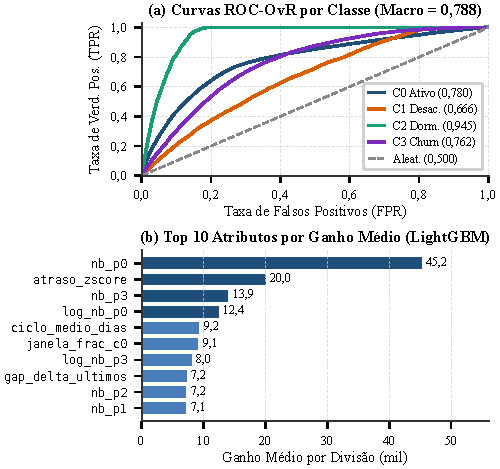
\includegraphics[width=0.91\columnwidth]{figs/fig3_roc_e_atributos.pdf}
\caption{Avaliação complementar do modelo final: (a) curvas ROC-OvR por classe e (b) 10 atributos de maior ganho médio no LightGBM.}
\label{fig:roc_imp}
\end{figure}

\section{Estratégia Final}
No Kaggle, os 25.691 clientes de teste dividem-se em 30\% no \textit{Public Leaderboard} ($n=7.707$) e 70\% no \textit{Private Leaderboard} ($n=17.984$). Testes \textit{bootstrap} na validação apontaram variação amostral esperada de $\pm 0{,}0074$ no placar público contra $\pm 0{,}0042$ no privado. Como o conjunto público é menor, baseamos a escolha na validação aninhada de 10 partições e na semelhança entre treino e teste (AUC adversarial de 0,5007). As duas submissões selecionadas são:
\begin{enumerate}
\item \textbf{\texttt{submissao\_v4\_10fold\_ensemble.csv} (Principal):} comitê linear calibrado com máscara estrutural e ajuste \textit{Plug-in} sem consultar rótulos externos ($\text{F1 CV}=0{,}4398$; $\text{AUC}=0{,}7880$; \textbf{0,44075} no \textit{Public LB});
\item \textbf{\texttt{submissao\_v4\_10fold\_melhor\_individual.csv} (Salvaguarda):} modelo único \textit{CatBoost Hierárquico Nativo} em 10 partições ($\text{F1 CV}=0{,}4370$; $\text{AUC}=0{,}7874$; \textbf{0,43716} no \textit{Public LB}), opção segura contra variações nos pesos de mistura no conjunto privado.
\end{enumerate}
Ambas foram auditadas com 25.691 linhas, zero ausentes, proporções consistentes ($\approx 26{,}0\% / 8{,}4\% / 4{,}5\% / 61{,}2\%$) e 96,15\% de concordância.

\section{Conclusões}
Os experimentos mostraram que pré-processamento e pós-processamento pesam tanto quanto o classificador escolhido. Preservar clientes legítimos ante filtros IQR ($+0{,}0098$), criar 170 atributos com BG/NBD sem vazamento, adotar decomposição hierárquica com tratamento nativo no CatBoost e ajustar limiares com \textit{Plug-in} elevou o F1-macro de 0,3389 para \textbf{0,4398} na validação cruzada (\textbf{0,44075} no \textit{Public LB}), a 0,0009 do limite Bayesiano estimado.

A principal limitação observada foi a dificuldade em separar a Classe~1 das classes vizinhas com apenas nove meses pré-corte. Como extensões futuras em Aprendizado de Máquina, sugerimos bases plurianuais para capturar sazonalidade completa, modelos de análise de sobrevivência para estimar tempo contínuo até a próxima compra e redes neurais específicas para dados tabulares mistos.

\FloatBarrier

\bibliographystyle{IEEEtran}
\bibliography{referencias}

\end{document}
